\chapter{原初双黑洞并合率}\label{chap:mergerrate}

\section{背景介绍}

%Up to now several gravitational-wave events from the coalescences of black hole binaries have been reported by LIGO/VIRGO, and imply that black holes should have an extended mass function. We work out the merger rate distribution of primordial-black-hole binaries with a general mass function by taking into account the torques by all primordial black holes and linear density perturbations. In the future, many more coalescences of black hole binaries are expected to be detected, and the one-dimensional and two-dimensional merger rate distributions will be crucial for reconstructing the mass function of primordial black holes. 

人们普遍认为在宇宙早期,由于密度涨落的塌缩,有可能形成原初黑洞\cite{Hawking:1971ei,Carr:1974nx,Carr:1975qj}。另外,理解暗物质的本性到底是什么,依然是困扰物理学界的一大难题。作为暗物质的候选者之一,原初黑洞近年来吸引了越来越多的关注。这是因为原初黑洞不仅可能构成部分或全部的暗物质,而且LIGO-Virgo科学组织探测到的引力波事件\cite{Abbott:2016blz}可能就来源于原初双黑洞的并合\cite{Sasaki:2016jop,Bird:2016dcv}。

根据LIGO-Virgo科学组织最新发布的引力波瞬变目录2\cite{Abbott:2020niy},目前一共探测到了50个致密双星并合事例。其中大多数都是双黑洞并合的事例。引力波的观测表明,黑洞应当有质量分布,而不是单一质量的。事实上,形成原初黑洞的初始条件也表明原初黑洞的质量谱应当有一定的宽度。

在文献中,主要有两种原初双黑洞的形成机制。在第一种机制中,原初双黑洞形成于早期宇宙 \cite{Sasaki:2016jop,Nakamura:1997sm,Ali-Haimoud:2017rtz};而在另一种机制中,原初双黑洞形成于晚期宇宙 \cite{Bird:2016dcv,Ali-Haimoud:2017rtz,Nishikawa:2017chy}。研究表明,原初双黑洞的并合率主要由第一种机制主导。在过去的研究中,人们通常假定所有原初黑洞的质量都是一样的,即假定原初黑洞的质量谱是单色的\cite{Sasaki:2016jop,Nakamura:1997sm,Ali-Haimoud:2017rtz,Bird:2016dcv,Nishikawa:2017chy}。最近,文献\cite{Raidal:2017mfl}和文献\cite{Kocsis:2017yty}计算了有质量分布的原初双黑洞的并合率。但他们的计算都有可以改进的地方。例如,文献\cite{Raidal:2017mfl}只考虑了距离原初双黑洞系统最近的第三个黑洞对双黑洞系统的潮汐作用,而忽略了其他黑洞对双黑洞系统的相互作用;文献\cite{Kocsis:2017yty}只考虑了平的原初黑洞质量谱,而且质量谱的宽度很窄。

在这章中,我们将计算最一般质量谱下的原初双黑洞的并合率。在计算过程中,我们将考虑所有其他原初黑洞以及线性物质密度扰动对原初双黑洞系统产生的力矩。在未来的几十年内,我们将探测到越来越多的双黑洞并合事件,进而获取更多的黑洞质量分布的信息。利用黑洞质量分布的信息以及理论模型推演出来的并合率,我们将有可能回答引力波探测到的黑洞的起源以及这些黑洞是如何演化的。

\section{有质量分布情况下的原初双黑洞并合率的计算}
我们将原初黑洞的质量分布函数记作$P(m)$,其满足归一化条件
\e
\int_0^\infty P(m)dm=1.
\q
同时,在质量区间$(m, m+dm)$内的原初黑洞占冷暗物质的丰度为
\e
f_\mathrm{tol} P(m)dm, 
\q
其中$f_\mathrm{tol}$是原初黑洞占非相对论物质的总丰度。为了方便,我们以太阳质量$M_\odot$作为原初黑洞质量的单位。原初黑洞占冷暗物质的丰度和$f_\mathrm{tol}$的关系为$\fpbh\equiv \Omega_{\rm{PBH}}/\Omega_{\rm{CDM}} \approx f_\mathrm{tol}/0.85$。为了方便,我们将质量分布函数做离散化,即
\e
\int P(m)dm=1\ \rightarrow \ \sum_{m_{\rm{min}}\leq m_i \leq m_{\rm{max}}} P_i \Dt \simeq 1, 
\q
其中$P(m_i) \rightarrow P_i$是粗粒化的质量分布函数,而$dm_i \rightarrow \Dt$是原初黑洞质量的微小单元。简单来说,质量为$m_i$的原初黑洞的丰度即为$f P_i \Dt\equiv f_i \Dt$。在辐射-物质平衡时期,总的能量密度为
\e
\rhoeq =\Omega_m \rho_{\rm{crit}} (1+z_{\rm{eq}})^3, 
\q
而两个质量为$m_i$的原初黑洞之间的平均距离$\xbar_i$为
\e
\xbar_i = \({3\over 4\pi} {m_i\over \rhoeq f_i \Dt}\)^{1/3}.
\q
需要注意的是,$\xbar_i$不仅取决于原初黑洞的质量$m_i$,而且取决于该质量的原初黑洞的丰度$f_i \Dt$。需要强调的是,不同质量的原初黑洞的数密度可以极不相同的。所以对所有原初黑洞来说,并没有良好定义的数密度概念。对于两个邻近但质量不同的原初黑洞,假定其质量分别为$m_i$和$m_j$,则它们的平均距离为
\e
\langle x_{ij}\rangle=  \(\xbar_i^{-3}+\xbar_j^{-3}\)^{-1/3}
= \mu_{ij}^{1/3} \xbar_{ij}, 
\q
其中 
\m
\mu_{ij}&=& {2m_im_j f_{b}\over m_{b}(f_jm_i+f_im_j)},\label{mu}\\
\xbar_{ij}^3&=&{3\over 8\pi} {m_{b}\over \rhoeq f_{b} \Dt}, %\equiv {{\tilde x}_{ij}^3\over \Dt}, 
\label{xbar}
\n
并且 
\m
f_{b}&=&f_i+f_j,\\
m_{b}&=&m_i+m_j. 
\n 
需要注意的是,以上公式只有当两个原初黑洞具有不同质量,即$m_i\neq m_j$时才成立。当$m_i=m_j=m$时,需要做如下替换$P(m_i)=P(m_j)=P(m)/2$。 
在本章中,在不会混淆的情况下,我们去掉下标`$_{ij}$'。

下面我们考虑原初双黑洞的形成和演化过程。在宇宙早期,两个邻近的原初黑洞需要从宇宙膨胀的背景中退耦出来才能形成双黑洞束缚系统。假设质量为$m_i$和$m_j$的两个原初黑洞沿着运动方向的固有距离为$r$,则在在牛顿近似下,$r$需要满足以下运动方程
\e\label{eom1}
\ddot{r} - \( \dot{H} + H^2 \) r + \frac{m_b}{r^2} \frac{r}{|r|} = 0, 
\q
其中一点表示对固有时间的导数。在本章中,我们使用几何单位制,即要求牛顿常数$G$和光速$c$满足$G=c=1$。

假设两个原初黑洞的共动距离为$x$。为了方便,我们定义$\chi \equiv r/x$。则公式\eqref{eom1}可以改写为
\e
\chi'' + \frac{s h' + h}{s^2 h} \(s \chi' - \chi \) + \frac{1}{\la}
\frac{1}{\(sh\)^2} \frac{1}{\chi^2} \frac{\chi}{|\chi|} = 0, 
\label{chi}
\q
其中一撇代表对尺度因子$s$的导数。我们将尺度因子在辐射-物质平衡时期的大小定为1。公式\eqref{chi}的$h(s)$定义为$h(s)\equiv H(s)/\({8\pi\over 3}\rhoeq\)^{1/2}=\sqrt{s^{-3}+s^{-4}}$。这里的$\la$是一个无量纲的参数,其定义为
\e
\la = \frac{8 \pi \rhoeq x^3}{3 m_b} = {X\over f_b\Dt},
\q
其中
\e
X\equiv {x^3/\xbar^3}, 
\q
其中$\xbar$由公式\eqref{xbar}给出。由公式\eqref{chi}的解可以看出如果$\lambda<1$则退耦会发生在辐射-物质平衡之前\cite{Ali-Haimoud:2017rtz}。另外,双黑洞系统的半长轴$a$的解为
\e
a \approx 0.1 \la x = \frac{0.1}{f_b \Dt} \frac{x^4}{\xbar^3}
={0.1 \xbar \over f_b\Dt} X^{\frac{4}{3}}. 
\label{axis}
\q 

如果没有其他黑洞或者密度扰动提供潮汐力,双黑洞则会直接迎头碰撞而并合。如果有潮汐力的话,那么潮汐力会为双黑洞系统提供角动量,从而使得双黑洞形成束缚系统,而不是直接并合。为了方便,我们引入一个无量纲的角动量$j$,其定义为 
\e
j\equiv \ell/\sqrt{m_b a}=\sqrt{1-e^2}, 
\q
其中$\ell$为单位约化质量的角动量。另外$e\in[0,1]$为偏心率。下面的关键问题乃是估计初始轨道的参数。我们推广了文献\cite{Ali-Haimoud:2017rtz}中的方法来估算两个具有不同质量的原初黑洞构成的双黑洞系统的初始轨道参数。下面我们给出简要的推导过程。

假设牛顿势为$\phi$,则局域的潮汐场为$T_{ij}=-\p_i\p_j \phi$。潮汐场会产生潮汐力。对每单位质量,潮汐力的大小为$\mathbf{F}=\mathbf{T}\cdot \mathbf{r}$。由于双黑洞系统的初始共动距离要比平均距离小很多,所以潮汐力并不会对双黑洞的轨道有很大的影响。潮汐力会产生力矩,其大小为
\e
\mathbf{\ell}=\int dt\ \mathbf{r}\times [\mathbf{T}\cdot \mathbf{r}]. 
\q
由于在辐射主导时期,其他原初黑洞以及密度涨落产生的潮汐场正比于$s^{-3}$,即$\mathbf{T}\simeq s^{-3} \mathbf{T}_{\rm{eq}}$,所以角动量为
\e\label{angular_j}
\bj \approx x^3 \hx \times \[\frac{\mathbf{T}_{\rm{eq}}}{m_b} \cdot \hx \], 
\q
其中$\hx$是沿着$\mathbf{x}$方向的单位矢量,而$\mathbf{T}_{\rm{eq}}$是在辐射-物质平衡时期的局域潮汐场。现在考虑质量为$m_l$的第三个原初黑洞。假设这个黑洞与双黑洞的距离$y$远远大于双黑洞的距离$x$,即$y\gg x$,则第三个黑洞产生的潮汐场为
\e
T^{ij}_{eq} = m_l \frac{3 \hy^i \hy^j - \dt^{ij}}{y^3},
\q
其中$\hy$是沿着$\mathbf{y}$方向的单位矢量。\eqref{angular_j}式进而可以变为
\e
\mathbf{j} \approx 3 \frac{m_l}{m_b} \frac{x^3}{y^3} 
\(\hx \cdot \hy\) \(\hx \times \hy\).
\q
与文献\cite{Ali-Haimoud:2017rtz}类似,下面我们参照\cite{Chandrasekhar:1943ws}来计算角动量的概率分布函数。所有其他黑洞产生的角动量$j$的二维概率密度函数为
\e
\frac{dP}{d^2 j} = \lim_{V \to \infty}\int \frac{d^2 k}{\(2\pi\)^2} e^{i \mathbf{k} \cdot \bj} 
\prod_{l} {\cal I}_l^{N_l},
\q
其中$N_l=n_l V$是所有质量为$m_l$的原初黑洞的数目。另外,${\cal I}_l$为
\e
{\cal I}_l = \int_V \frac{d^3 y}{V} \exp\[-3 \frac{m_l}{m_b} i
\frac{x^3}{y^5} y_{||}\, \mathbf{k} \cdot \mathbf{y}_{\perp}\],
\q
其中$y_{||}$和$\mathbf{y}_{\perp}$分别定义为$y_{||}\equiv \mathbf{y}\cdot \hx$, $\mathbf{y}_{\perp}\equiv \hx\times \mathbf{y}$。经过繁琐的计算,我们会得到
\m
\lim_{V \to \infty} {\cal I}_l^{N_l} = e^{-{4\pi\over 3} {m_l\over m_b} n_l x^3 k}. 
\n
由于所有质量为$m_l$的原初黑洞的能量密度为$m_l n_l=\rho_l$,并且$\sum_l \rho_l=\rho_{\rm{pbh}}=f \rhoeq$,所以我们可以得到
\m\label{prob1}
\frac{dP}{dj} = j \int k dk J_0(kj) e^{-j_X k},
\n 
其中
\m
j_X=0.5{f\over f_b\Dt} X.
\n
$j_X$表征了所有其他原初黑洞产生的力矩的总和。对公式\eqref{prob1}积分会得到
\m\label{Pj}
\left. j \frac{dP}{dj} \right\vert_X = \mP\(j/j_X\), \quad
\mP(\ga) = \frac{\ga^2}{\(1 + \ga^2\)^{3/2}},
\label{pj}
\n
其中$\gamma=j/j_X$。此外,密度涨落产生的力矩$\mathbf{j}$的方差为
\e
\langle j^2 \rangle^{1/2}\approx 0.5 {8\pi\over 3} {\sigma_{\rm{eq}}\rhoeq \over m_b}x^3=0.5 {\sigma_{\rm{eq}}\over f_b\Dt} X, 
\q
其中$\sigma_{\rm{eq}}\equiv \langle \delta_{\rm{eq}}^2 \rangle^{1/2}$是其他暗物质在辐射-物质平衡时期在${\cal O}(10^0\sim10^3) M_\odot$尺度上的密度涨落的方差。考虑到所有其他原初黑洞以及密度涨落产生的力矩,那么\eqref{pj}式中的$j_X$的特征大小为 
\e
j_X\approx 0.5 \(f^2+\sigma_{\rm{eq}}^2\)^{1/2} {X\over f_b\Dt}. 
\label{jx}
\q

在形成原初双黑洞系统后,由于引力波辐射,双黑洞系统的轨道会收缩,最后并合。双黑洞的并合时间由系统的质量、轨道距离以及角动量共同决定,具体为\cite{Peters:1964zz}
\m 
t = \frac{3}{85} \frac{a^4}{m_i m_j m_b} j^7.
\n 
考虑到公式\eqref{axis},则无量纲的的角动量为
\m 
j(t; X) = \( \frac{85}{3} \frac{t m_i m_j m_b (f_b\Dt)^4}
{\(0.1\xbar\)^4 X^{16/3}} \)^{1/7}.
\n  
假设所有原初黑洞在空间上是随机分布的,则两个为$m_i$和$m_j$的最相邻原初黑洞的距离为$x$,且在体积${4\pi \over 3}x^3$内没有其他原初黑洞的概率为
\m 
% \frac{dP}{d{\tilde X}} = e^{- {\tilde X}},
\frac{dP}{d{\tilde X}} = e^{- {4\pi \over 3}x^3 n_T}=e^{- {\tilde X}\cdot {4\pi \over 3}\langle x_{ij} \rangle^3 n_T}, 
\label{dpX}
\n 
其中${\tilde X}\equiv x^3/\langle x_{ij} \rangle^3=X/\mu$,而$\mu$由公式\eqref{mu}给出,并且$n_T\equiv f\rho_{\rm{eq}}\int_0^\infty {P(m)\over m}dm$。如果$m_i\approx m_j$,则$\mu\approx 1$。但是如果两个原初黑洞的质量比很大的话,那么$\mu$可以远远小于$1$,那么文献\cite{Ali-Haimoud:2017rtz}中给出的近似表达式$dP/dX\approx 1$ 将不再有效。需要注意的是,我们推广了文献\cite{Ali-Haimoud:2017rtz}计算单一质量原初黑洞的结果,我们发现在有质量分布的情况下,在指数项会有一个$1/\mu$因子的修正。在$m_i = m_j$的特例下,$\mu = 1$,进而我们的结果退回到文献\cite{Ali-Haimoud:2017rtz}的结果。然而,对于极端质量比的双黑洞系统,这个因子可能会产生很大影响,进而导致文献\cite{Ali-Haimoud:2017rtz}使用的近似表达式$e^{- X/\mu} \app 1$不再有效。利用关系式$j \propto t^{1/7}$,$\p j/\p t = j/(7t)$和公式\eqref{Pj},我们得到
\e
\frac{d^2 P}{d{\tilde X} dt} = \frac{1}{7 t} e^{- {\tilde X}\cdot {4\pi \over 3}\langle x_{ij} \rangle^3 n_T}\, \mP(\ga_X),
\quad \ga_X \equiv \frac{j(t; X)}{j_X}, 
\q 
其中$j_X$由公式\eqref{jx}给出。对上式的$\tilde{X}$进行积分,我们可以到并合时间的概率分布函数
\e 
\frac{dP}{dt}  %\int \frac{d{\tilde X}}{7 t}  e^{- {\tilde X}\cdot {4\pi \over 3}\langle x_{ij} \rangle^3 n_T} \mP(\ga_X) \nonumber\\
= \frac{\mu^{-1}}{7 t} \int d{X} e^{- {X\over \mu}\cdot {4\pi \over 3}\langle x_{ij} \rangle^3 n_T} \mP(\ga_X),
\label{dP}
\q
进而在时间$t$时,原初黑洞的共动并合率为
\m
R_{ij}(t)\equiv {dN_{\rm{merger}}\over dtdV}=\rho_m^0 \min\(\frac{f_i \Dt}{m_i}, \frac{f_j \Dt}{m_j}\) {dP\over dt}, 
\n
其中$\rho_m^0\simeq 4\times 10^{19}\, \Msun \text{Gpc}^{-3}$为今天的物质密度。概率函数${\cal P}(\gamma_X)$有一个很尖的峰,其尖峰的位置为
\e
X_*(t)\approx 0.032 \({t\over t_0}\)^{3\over 37} f_b \Delta (f^2+\sigma_{\rm{eq}}^2)^{-{21\over 74}} (m_i m_j)^{3\over 37} m_b^{-{1\over 37}}.
\q
由于${X_*\over \mu}\cdot {4\pi \over 3}\langle x_{ij} \rangle^3 n_T\ll 1$, 所以在$t$时刻的共动并合率为
\m
R_{ij}(t)= {\cal R}_{ij}(t) \Delta^2, 
\n
其中  
\m
{\cal R}_{ij}(t)&\approx& 3.9\cdot 10^6\times  \({t\over t_0}\)^{-{34\over 37}} f^2 (f^2+\sigma_{\rm{eq}}^2)^{-{21\over 74}} \nonumber \\
&\times&  \min\(\frac{P(m_i)}{m_i}, \frac{P(m_j)}{m_j}\) \({P(m_i)\over m_i}+{P(m_j)\over m_j}\) \nonumber \\
&\times& (m_i m_j)^{{3\over 37}} (m_i+m_j)^{36\over 37}.
\n
${\cal R}_{ij}(t)$是以Gpc$^{-3}$ yr$^{-1}$为单位的共动并合率密度分布。需要注意到是,本章中原初黑洞的质量是以太阳质量$M_\odot$为单位的。需要再次强调的是,在$m_i=m_j=m$时,$P(m_i)=P(m_j)=P(m)/2$。文献\cite{Kocsis:2017yty}定义了一个量$\tilde{\alpha} \equiv -(m_i+m_j)^2\p^2 \ln {\cal R}_{ij}/\p m_i \p m_j$,且认为$\tilde{\alpha}$的值应该约等于$36/37$。如果$P(m)/m=$是个常数的话,那么$\tilde{\alpha}=36/37$,则和文献\cite{Kocsis:2017yty}的结果吻合。但是对于一个一般的质量函数分布,$\tilde{\alpha}$可以不同于$36/37$。

\section{与引力波数据的比较}
下面我们考虑文献中经常用到的两个原初黑洞的质量函数分布。第一个是幂率分布\cite{Carr:1975qj}
\m
P(m)\approx {\alpha-1\over M} \({m\over M}\)^{-\alpha}
\n
其中$m\geq M$,且$\alpha>1$。第二个为对数正态分布\cite{Dolgov:1992pu}
\m
P(m) = \frac{1}{\sqrt{2 \pi} \sigma m} 
\exp\(-\frac{\ln^2(m/m_c)}{2 \sigma^2}\), 
\n
其中$m_c$表征质量谱的峰值,而$\s$表征质量谱的宽度。
在文献\cite{Abbott:2017vtc}中,LIGO-Virgo科学组织限制了质量范围在$m_1,\ m_2\geq 5M_\odot$和 $m_1+m_2\leq 100M_\odot$内的双黑洞的并合率大小$R_T$,要求$12 \lesssim R_T \lesssim 213$ Gpc$^{-3}$ yr$^{-1}$。与文献\cite{Ali-Haimoud:2017rtz}一样,我们取$\sigma_{\rm{eq}}\approx 0.005$。在图\ref{merger}我们列出了这两种质量分布下的并合率随着原初黑洞丰度的关系。其中粉红色区域是LIGO-Virgo科学组织给出的并合率的范围。在这个图中,对于幂率质量分布函数,我们选取$M=5\Msun$和$\alpha=1.6$;而对于对数正态质量分布函数,我们选取$m_c=15M_\odot$和$\sigma=0.6$。从这个图可以看出,用原初黑洞模型确实可以解释LIGO-Virgo科学组织探测的双黑洞。
从LIGO-Virgo科学组织给出的并合率限制,我们可以反推出原初黑洞占暗物质丰度$\fpbh$的限制。对于幂率形式的质量分布函数,$\fpbh$需要满足$1.4\times 10^{-3} \lesssim \fpbh \lesssim 6.6\times 10^{-3}$;而对于对数正态形式的质量分布函数,$\fpbh$需要满足$1.2\times 10^{-3} \lesssim \fpbh \lesssim 5.7\times 10^{-3}$。以上得到的$\fpbh$的限制和其他观测\cite{Chen:2016pud,Green:2016xgy,Schutz:2016khr,Wang:2016ana,Gaggero:2016dpq,Ali-Haimoud:2016mbv,Blum:2016cjs,Horowitz:2016lib,Kuhnel:2017pwq,Inoue:2017csr,Carr:2017jsz,Green:2017qoa,Guo:2017njn,Zumalacarregui:2017qqd,Clesse:2016vqa}给出来的是一致的。

\begin{figure}[htb]
    \centering
    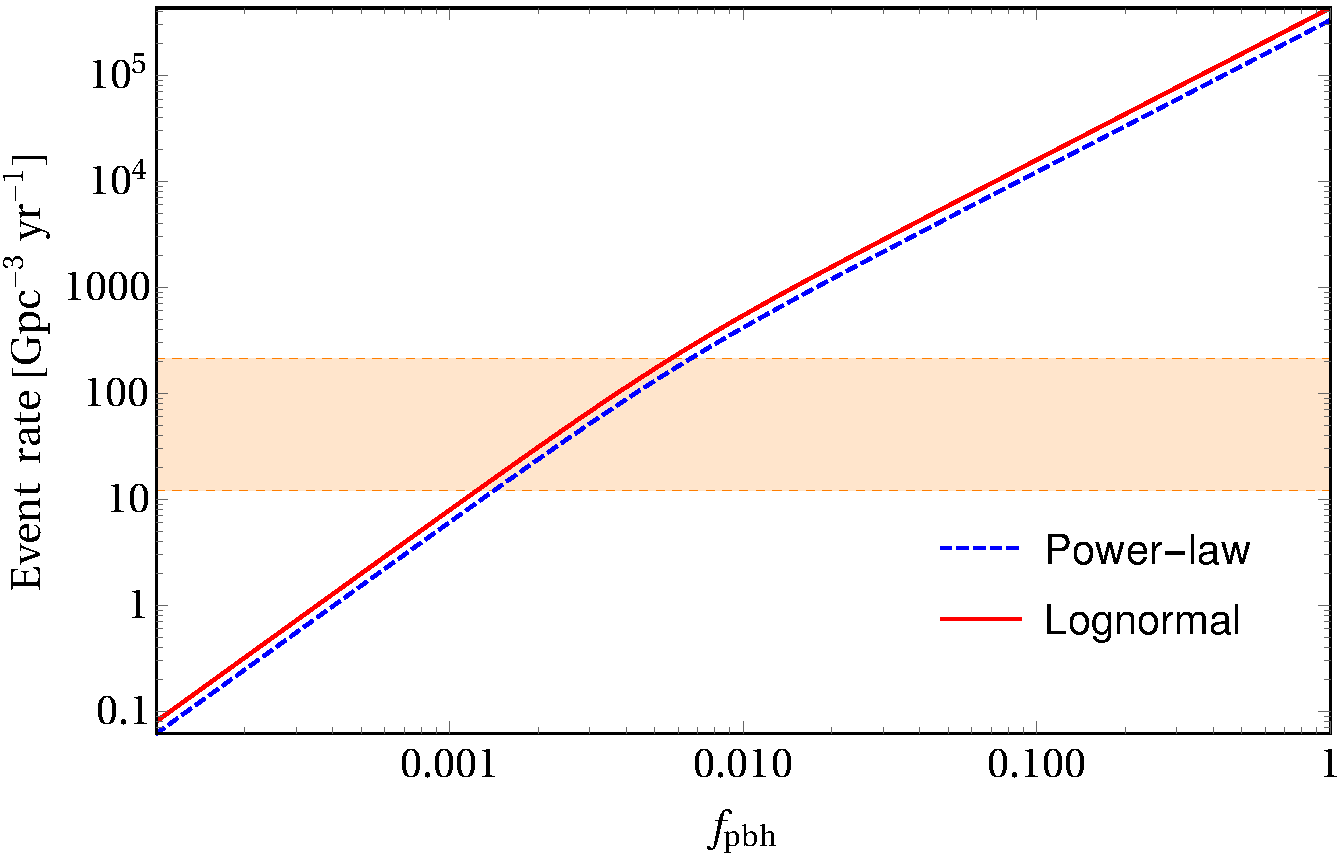
\includegraphics[width=0.86\textwidth]{mergerfpbh.pdf}
    \bicaption{ 
        在质量为$m_1,\ m_2\geq 5M_\odot$且$m_1+m_2\leq 100M_\odot$的范围内,今天的原初双黑洞的并合率和$\fpbh$的关系图。蓝色点线和红色实线分别对应为\textit{幂率}质量分布函数($M=5M_\odot$且$\alpha=1.6$)和\textit{对数正态}质量分布函数($m_c=15M_\odot$且 $\sigma=0.6$)。
    }{The merger rate of PBH binaries at present as a function of $\fpbh$ with $m_1,\ m_2\geq 5M_\odot$ and $m_1+m_2\leq 100M_\odot$. The blue dotted and red solid lines correspond to the \textit{power-law} mass distribution ($M=5M_\odot$ and $\alpha=1.6$) and \textit{lognormal} mass distribution ($m_c=15M_\odot$ and $\sigma=0.6$), respectively. }
    \label{merger}
\end{figure}

\begin{figure}[htb!]
    \centering
    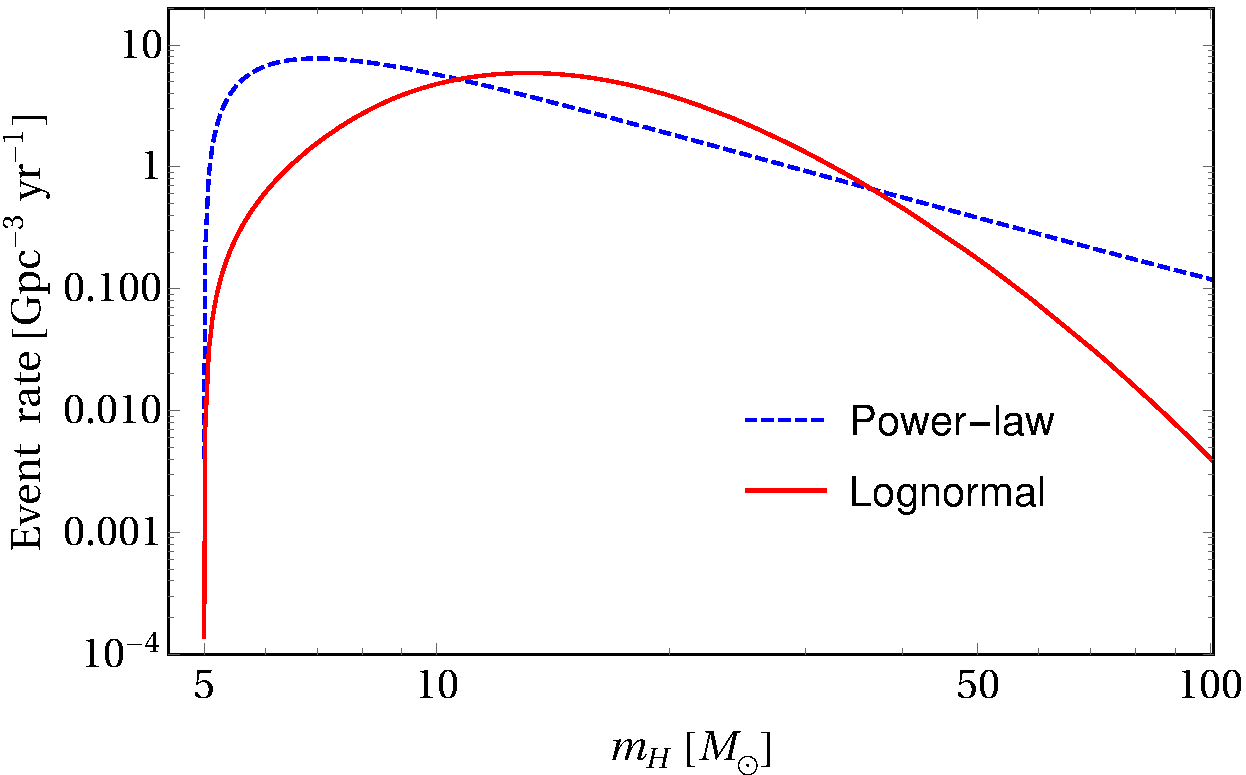
\includegraphics[width=0.86\textwidth]{mergerheavy.pdf}
    \bicaption{\label{mergerheavy}
        一维的并合率分布。其中$m_H$是双黑洞系统中较重黑洞的质量。我们把较轻黑洞的质量积分掉,积分范围为$5M_\odot$到$m_H$。蓝色实线对应的是$\fpbh =4.3\times 10^{-3}$时的\textit{幂率}形式的质量分布函数($M=5M_\odot$且$\alpha=1.6$);而红色实线对应的是$\fpbh = 3.7\times 10^{-3}$时的\textit{对数正态}形式的质量函数分布($m_c=15M_\odot$且$\sigma=0.6$)。
    }{The 1D merger rate distribution, where $m_H$ is the mass of heavier BH in the binary and the mass of lighter BH is integrated over from $5M_\odot$ to $m_H$. The blue dotted and red solid lines correspond to the \textit{power-law} PDF ($M=5M_\odot$ and $\alpha=1.6$) with $\fpbh =4.3\times 10^{-3}$ and \textit{lognormal} PDF ($m_c=15M_\odot$ and $\sigma=0.6$) with $\fpbh = 3.7\times 10^{-3}$, respectively.}
\end{figure}

从图\ref{merger}可以看出,不同的质量分布都能解释目前LIGO-Virgo得到的并合率限制。为了打破这种简并,我们需要更多的信息。假如固定总的并合率为$R_T=100$ Gpc$^{-3}$ yr$^{-1}$,对于幂率形式的质量函数,我们可以得到$\fpbh = 4.3\times 10^{-3}$;而对于对数正态形式的质量分布函数,我们可以得到$\fpbh = 3.7\times 10^{-3}$。在图\ref{mergerheavy}中,通过把较轻的黑洞质量积分掉,我们画出了一维的并合率分布。可以看出,尽管幂率形式的质量分布和对数正态形式的质量函数分布都能给出相同的总并合率$R_T$,然而它们对应的一维并合率分布却大不相同。在图\ref{density}中,我们给出了二维的并合率分布中,由此我们可以得到更多的信息。

为了将计算得到的并合率和LIGO-Virgo探测到的引力波事件作比较,我们需要考虑LIGO-Virgo引力波探测器的灵敏度。这是因为并不是所有发生并合的双黑洞事件都能被LIGO-Virgo探测到,只有那些辐射出来的引力波的频率正好处于LIGO-Virgo灵敏的频段才能被LIGO-Virgo探测到。由于现阶段LIGO-Virgo能够探测到的并合事件的红移$z$大概在$z \in [0,1]$,所以预计能探测到的事件数$\Lambda$大致为\cite{Abbott:2016nhf,Abbott:2016drs,Abbott:2017iws,Kavanagh:2018ggo}
\e\label{lambda}
\Lambda_{ij} = \int_{0}^{1} R_{ij}(z) \frac{d\VT}{dz} dz,
\q 
其中$\VT$是LIGO-Virgo平均能探测到的时空体积。$\VT$不仅取决于探测器本身,而且还取决于双黑洞源的性质,比如双黑洞的质量大小。仿照\cite{Abbott:2016nhf,Abbott:2016drs,Usman:2015kfa,Veitch:2014wba},我们采取半解析的方法来计算$\VT$。在这里,我们假设LIGO的第一个观测阶段(O1)和第二观测阶段(O2)具有相同的空间体积。对于第一个探测阶段,其有$48.6$天的有效观测时间\cite{TheLIGOScientific:2016pea};而对于第二个探测阶段,其有$117$天的有效观测时间\cite{TheLIGOScientific:2017qsa}。需要注意的是,$\Lambda$并不是被探测到的双黑洞并合事件的平均数,而是超过一定阀值的事件数的平均值\cite{Abbott:2016nhf}。在这里我们取信噪比(SNR>8)作为可探测的阀值。在图\ref{events1}中,我们给出了二维的可探测事件数$\Lambda$的分布,以及LIGO-Virgo探测到的$6$个双黑洞并合事件。由于我们只用了有限的$6$个引力波事件,所以并不能最终确定哪个形式的质量分布函数和引力波数据拟合得更好。随着探测到双黑洞并合事件的累积,利用我们计算得到的原初黑洞并合率的分布,我们有可能确定黑洞质量函数的形式,以及黑洞质量到底有没有质量间隙\cite{Kovetz:2016kpi,Fishbach:2017zga}。

\begin{figure}[htb]
    \centering
    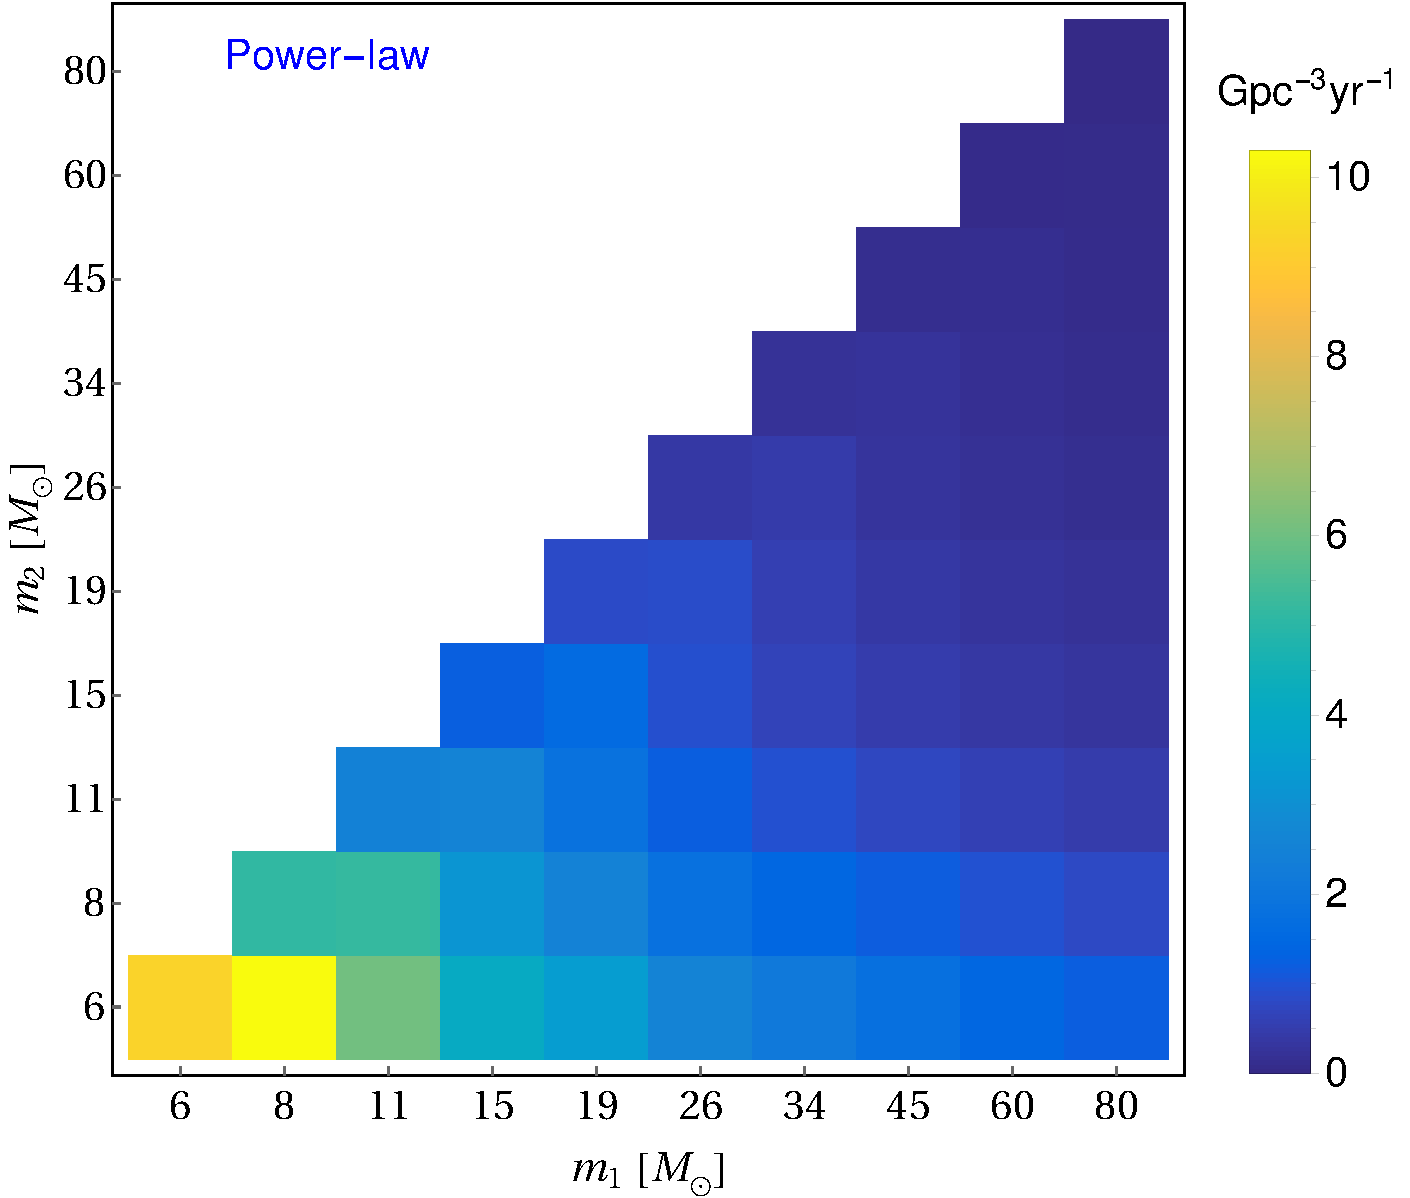
\includegraphics[width=0.8\textwidth]{binpower.pdf}\\
    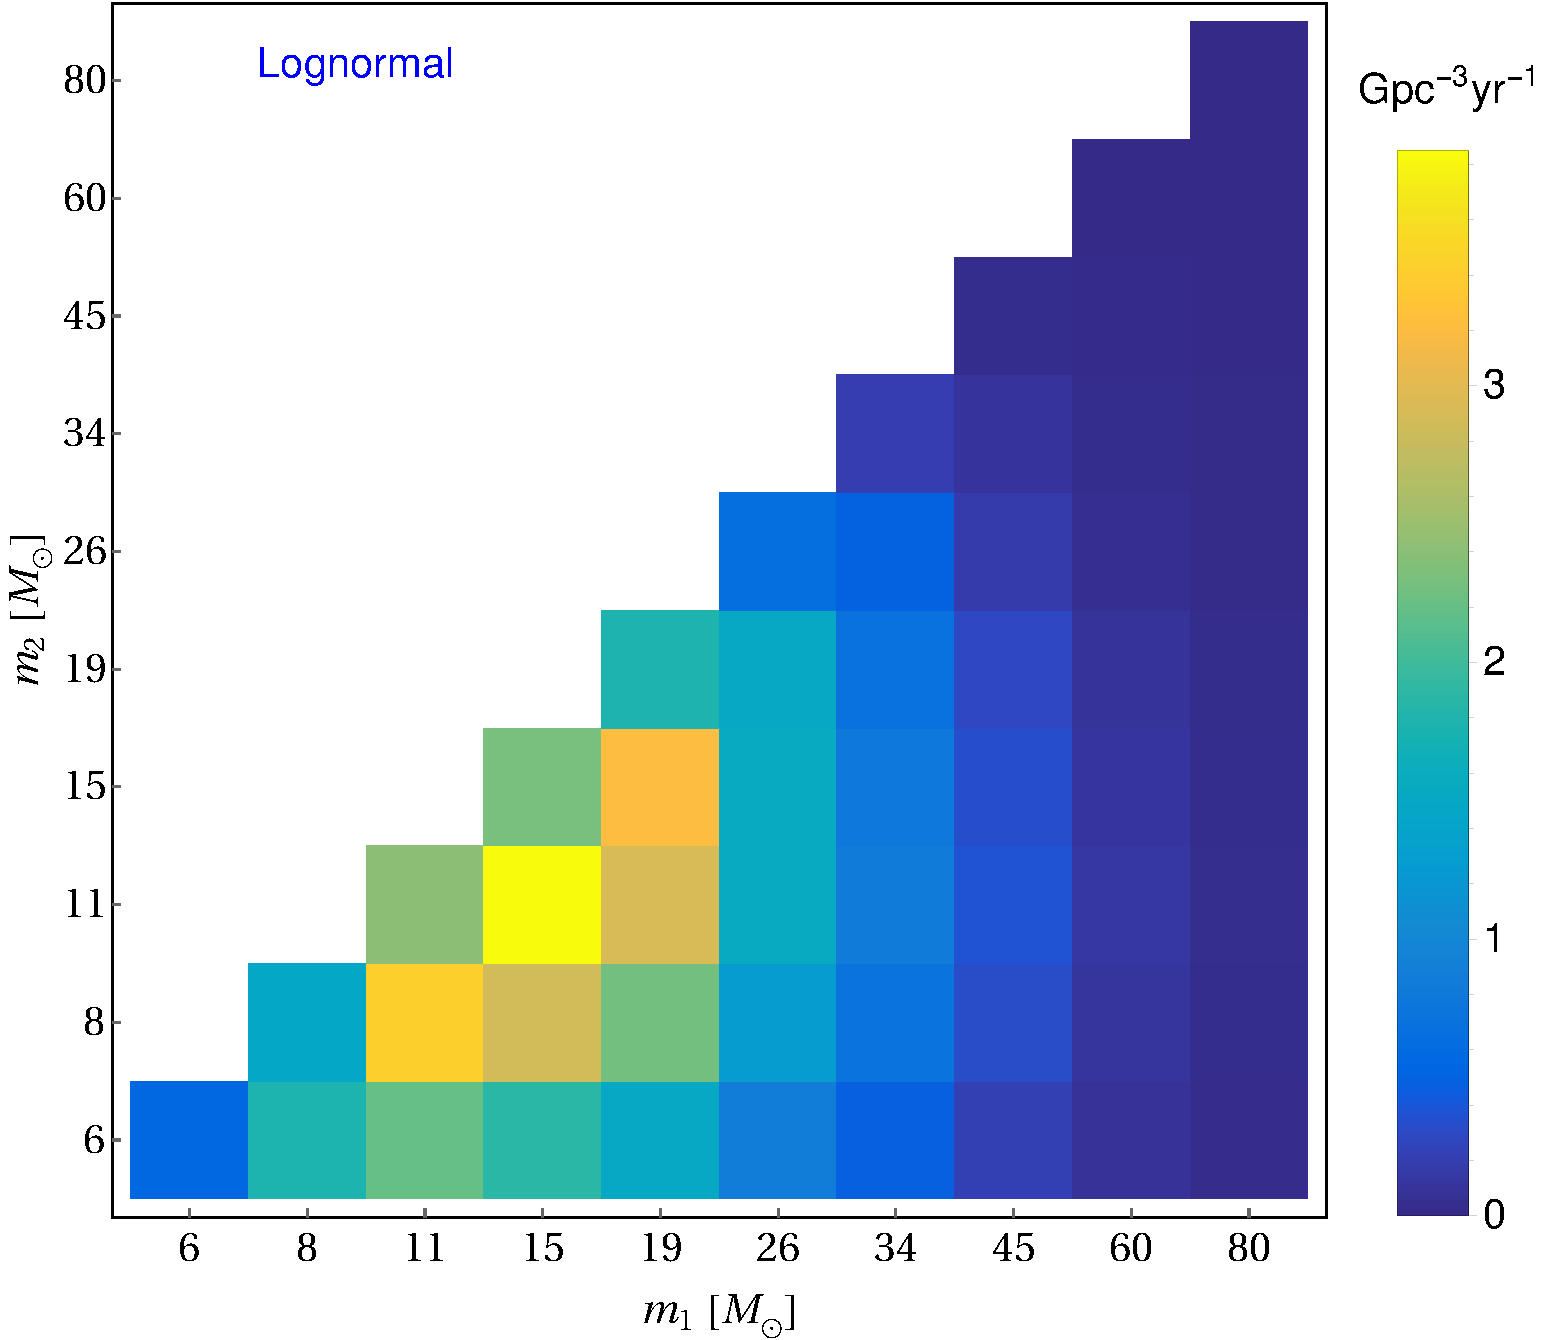
\includegraphics[width=0.8\textwidth]{binlog.pdf}
    \bicaption{\label{density}
        二维的并合率分布。上图对应的是$\fpbh = 4.3\times 10^{-3}$时的\textit{幂率}形式的质量函数($M=5M_\odot$且$\alpha=1.6$);而下图对应的是$\fpbh = 3.7\times 10^{-3}$时的\textit{对数正态}形式的质量函数($m_c=15M_\odot$且$\sigma=0.6$)。
    }{The 2D merger rate distributions. The top and bottom panels correspond to the \textit{power-law} mass function ($M=5M_\odot$ and $\alpha=1.6$) with $\fpbh = 4.3\times 10^{-3}$ and \textit{lognormal} mass function ($m_c=15M_\odot$ and $\sigma=0.6$) with $\fpbh = 3.7\times 10^{-3}$, respectively.}
\end{figure}

\begin{figure}[htb]
    \centering
    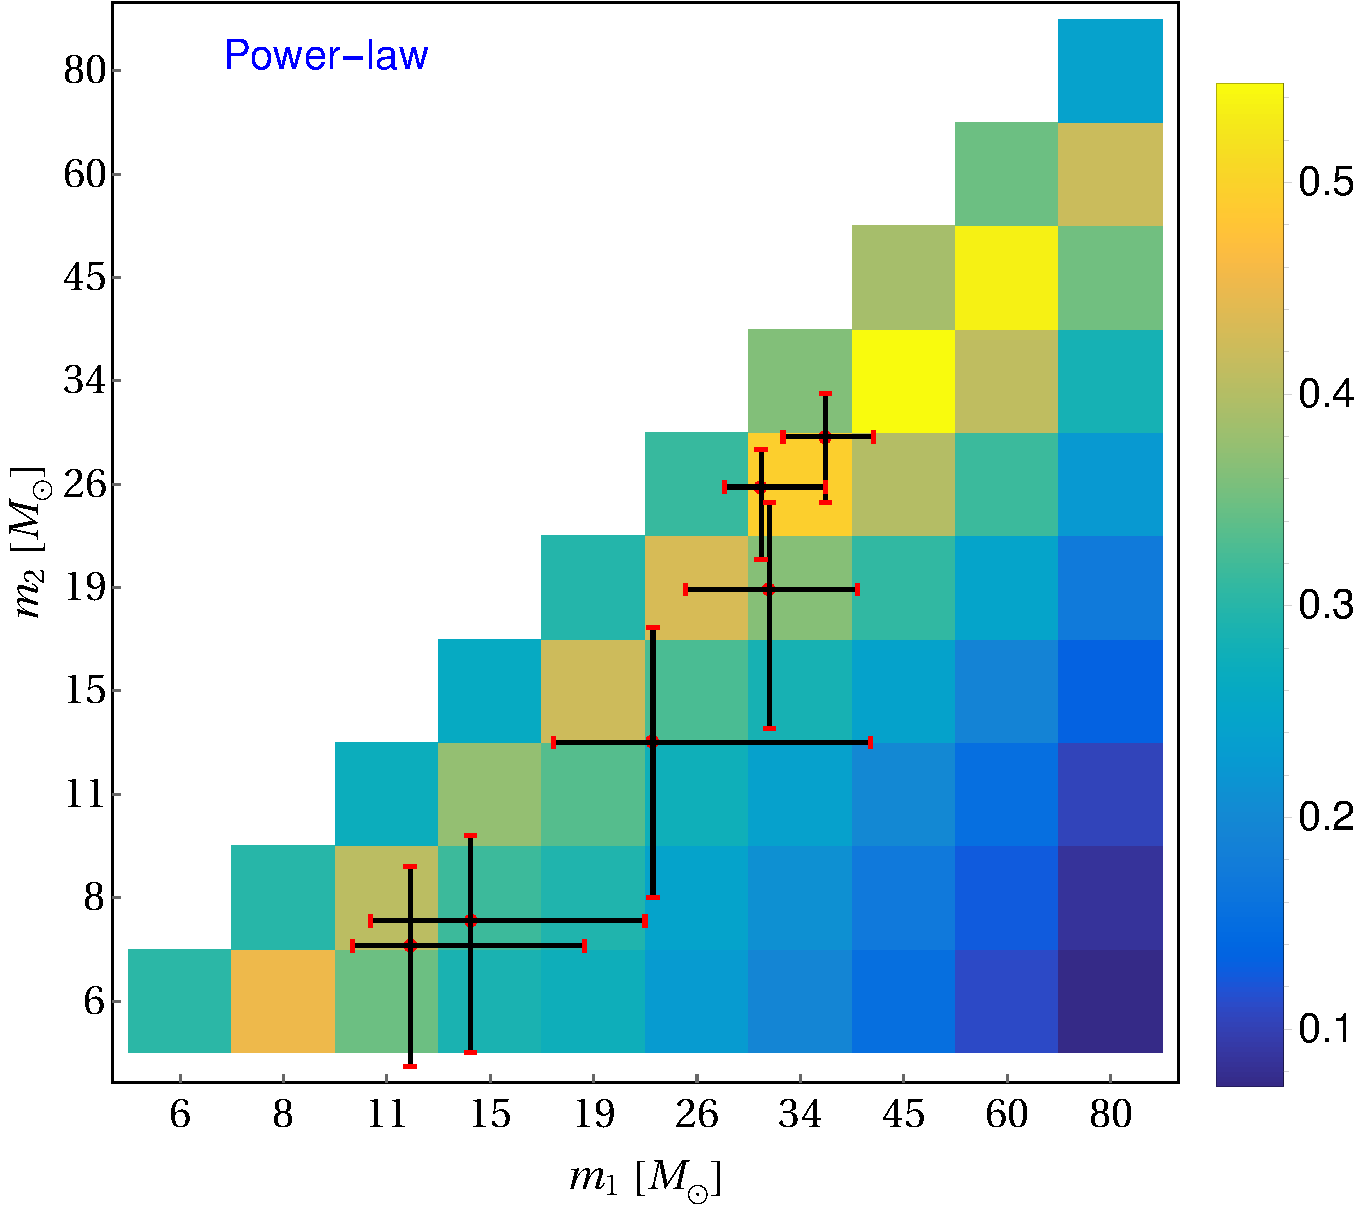
\includegraphics[width=0.72\textwidth]{binpowerrescale.pdf}
    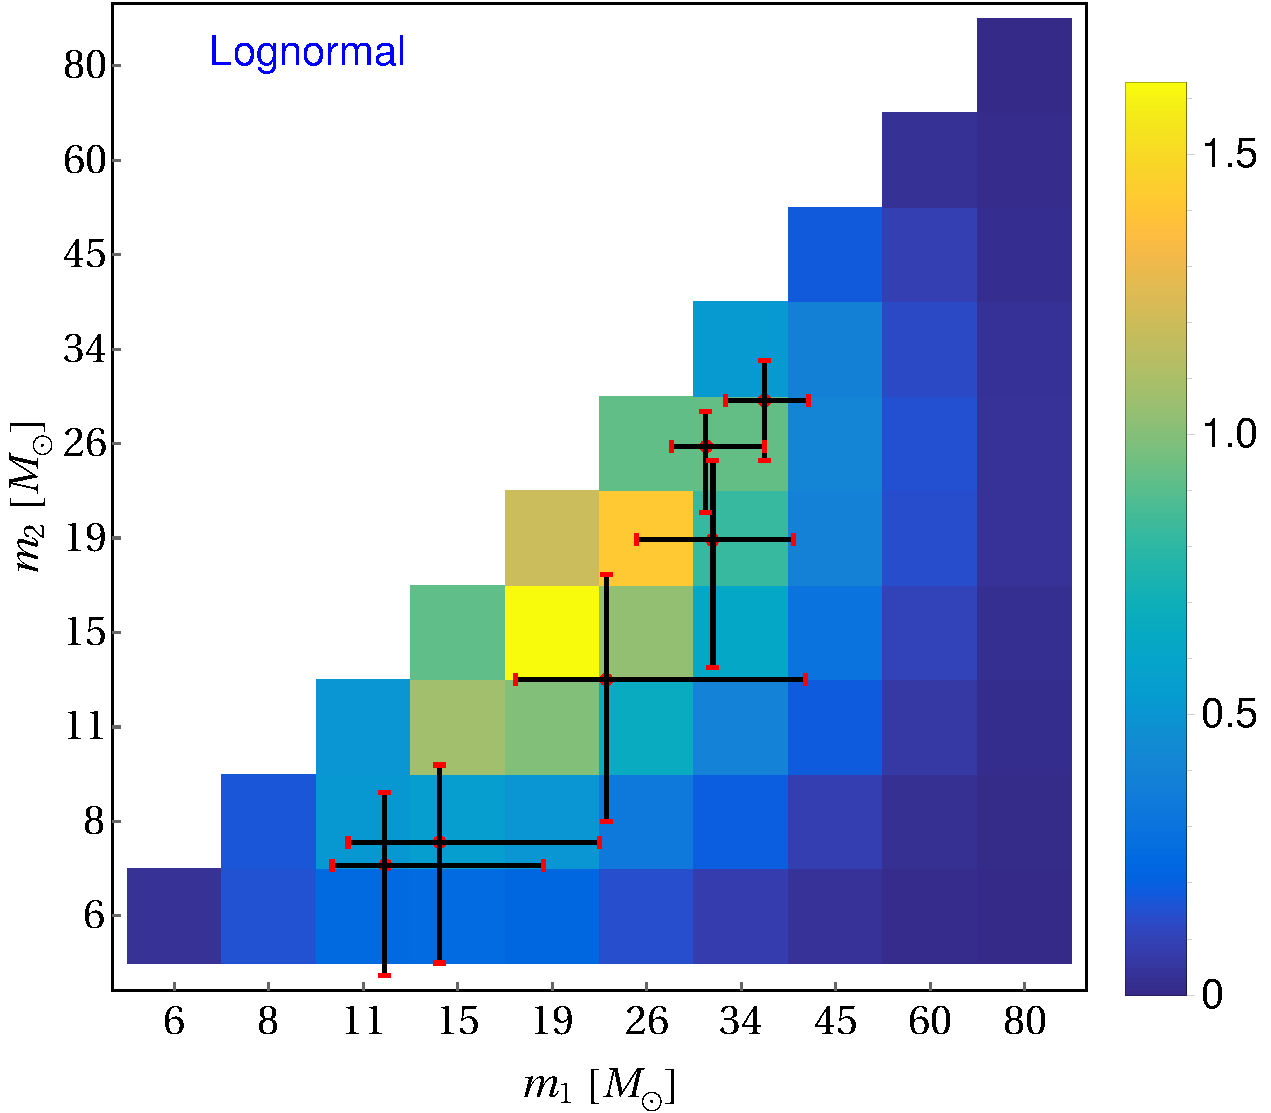
\includegraphics[width=0.72\textwidth]{binlogrescale.pdf}
    \bicaption{\label{events1}
        二维的可探测到的事件数$\Lambda$的分布[见公式\eqref{lambda}],以及LIGO-Virgo探测到的$6$个双黑洞并合事件。每个双黑洞并合事件的质量误差由图中的十字叉给出。上图对应的是$\fpbh = 4.3\times 10^{-3}$时的\textit{幂率}形式的质量函数($M=5M_\odot$且$\alpha=1.6$);而下图对应的是$\fpbh = 3.7\times 10^{-3}$时的\textit{对数正态}形式的质量函数($m_c=15M_\odot$且$\sigma=0.6$)。
    }{The 2D distributions for $\Lambda$ [see Eq.~\eqref{lambda}],
    along with the $6$ events detected by \lvc. 
    The crosses indicate error bars for each event.
    The top and bottom panels correspond to the \textit{power-law} 
    mass function ($M=5M_\odot$ and $\alpha=1.6$) with $\fpbh = 4.3\times 10^{-3}$
    and \textit{lognormal} mass function ($m_c=15M_\odot$ and $\sigma=0.6$) with $\fpbh = 3.7\times 10^{-3}$, respectively. }
\end{figure}

\section{本章小结}
在本章中,我们计算了具有一般质量分布情况下的原初双黑洞的并合率分布。在计算过程中,我们考虑所有其他原初黑洞以及线性密度扰动产生的力矩对原初双黑洞演化的影响。我们将计算得到的并合率分布与引力波数据做比较。我们分别考虑了幂率形式以及对数正态形式的原初黑洞的质量函数。对于幂率和对数正态形式的原初黑洞的质量函数,其对应的原初黑洞占暗物质的丰度$\fpbh$大概的量级为$10^{-3} \lesssim \fpbh \lesssim 10^{-2}$。我们得到的结果和其他观测\cite{Chen:2016pud,Green:2016xgy,Schutz:2016khr,Wang:2016ana,Gaggero:2016dpq,Ali-Haimoud:2016mbv,Blum:2016cjs,Horowitz:2016lib,Kuhnel:2017pwq,Inoue:2017csr,Carr:2017jsz,Green:2017qoa,Guo:2017njn,Zumalacarregui:2017qqd,Clesse:2016vqa}给出的结果是一致的,证实了绝大多数的暗物质不是由恒星级质量的原初黑洞构成的\cite{Sasaki:2016jop,Ali-Haimoud:2017rtz,Raidal:2017mfl,Kocsis:2017yty}。

目前有很多模型可以解释LIGO-Virgo探测到的双黑洞并合事件。观测这些双黑洞并合率的分布可能是区分原初黑洞模型和其他模型的一种强有力手段。我们发现原初双黑洞的并合率正比于$t^{-34/37}$。这是原初黑洞模型显著区别于其他模型的地方之一。此外,我们还发现一维和二维的并合率分布对原初黑洞的质量分布非常敏感。随着观测时间的增加以及引力波探测器的升级换代,未来我们可以观测到越来越多的双黑洞并合事件。利用一维和二维的原初黑洞并合率分布,我们有望重构出原初黑洞的质量分布,进而帮助我们理解LIGO-Virgo科学组织探测到的黑洞到底是怎么形成的,以及是如何演化的。